% Source : http://tex.stackexchange.com/questions/35989/tikz-connecting-nodeparts

\documentclass{article}
	\usepackage{tikz}
	\usetikzlibrary{shapes,positioning}


\begin{document}

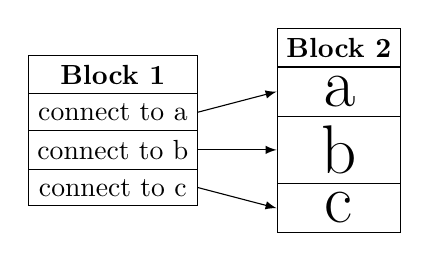
\begin{tikzpicture}
	\node[name=block, rectangle split, rectangle split parts=4, draw] {
		\textbf{Block 1}
		\nodepart{second} connect to a
		\nodepart{third} connect to b
		\nodepart{fourth} connect to c
	};

	\node[name=block2, rectangle split, rectangle split parts=4, draw, right= of block] {
		\textbf{Block 2}
		\nodepart{second} \Huge{a}
		\nodepart{third} \Huge{b}
		\nodepart{fourth} \Huge{c}
	};
	\draw [-latex] (block.two east) -- (block2.two west);
	\draw [-latex] (block.three east) -- (block2.three west);
	\draw [-latex] (block.four east) -- (block2.four west);
\end{tikzpicture}

\end{document}
